\documentclass[12pt,letterpaper]{article}
\usepackage{graphicx,textcomp}
\usepackage{natbib}
\usepackage{setspace}
\usepackage{fullpage}
\usepackage{color}
\usepackage[reqno]{amsmath}
\usepackage{amsthm}
\usepackage{fancyvrb}
\usepackage{amssymb,enumerate}
\usepackage[all]{xy}
\usepackage{endnotes}
\usepackage{lscape}
\newtheorem{com}{Comment}
\usepackage{float}
\newtheorem{lem} {Lemma}
\newtheorem{prop}{Proposition}
\newtheorem{thm}{Theorem}
\newtheorem{defn}{Definition}
\newtheorem{cor}{Corollary}
\newtheorem{obs}{Observation}
\usepackage[compact]{titlesec}
\usepackage{dcolumn}
\usepackage{tikz}
\usetikzlibrary{arrows}
\usepackage{multirow}
\usepackage{xcolor}
\newcolumntype{.}{D{.}{.}{-1}}
\newcolumntype{d}[1]{D{.}{.}{#1}}
\definecolor{light-gray}{gray}{0.65}
\usepackage{url}
\usepackage{listings}
\usepackage{color}
 
\definecolor{codegreen}{rgb}{0,0.6,0}
\definecolor{codegray}{rgb}{0.5,0.5,0.5}
\definecolor{codepurple}{rgb}{0.58,0,0.82}
\definecolor{backcolour}{rgb}{0.95,0.95,0.92}
 
\lstdefinestyle{mystyle}{
    backgroundcolor=\color{backcolour},   
    commentstyle=\color{codegreen},
    keywordstyle=\color{magenta},
    numberstyle=\tiny\color{codegray},
    stringstyle=\color{codepurple},
    basicstyle=\footnotesize,
    breakatwhitespace=false,         
    breaklines=true,                 
    captionpos=b,                    
    keepspaces=true,                 
    numbers=left,                    
    numbersep=5pt,                  
    showspaces=false,                
    showstringspaces=false,
    showtabs=false,                  
    tabsize=2
}
 \lstset{style=mystyle}
\newcommand{\Sref}[1]{Section~\ref{#1}}
\newtheorem{hyp}{Hypothesis}

\title{Text as Data: Homework 2}
\date{August 16, 2017}
\author{Jeff Ziegler}

\begin{document}
\maketitle

\noindent \textit{In this homework assignment we're going to compare the press releases of two senators---Richard Shelby and Jeff Sessions, Republican senators from Alabama.  To make this comparison, we're going to download a bigger collection of Senate press releases and then focus on the releases from Shelby and Sessions. We encourage you to spend some time processing these texts this week, because we will use this collection for the next homework assignment as well.}

\subsubsection*{Downloading the Data}

The press release collection are stored here:\\
{\tt https://github.com/lintool/GrimmerSenatePressReleases} \\

\noindent \textit{Download the collection as a {\tt .zip} file, unzip the file on your computer. } 

\subsubsection*{Creating a Document-Term Matrix}

\noindent \textit{We're going to use the files from Richard Shelby and Jeff Sessions to make two different kinds of Document-Term Matrices. The first will consider only the 1000 most used unigrams, while the second (separate) DTM will use the 500 most common trigrams. To create the document-term matrices, use the following recipe.}

\begin{itemize}
\item[1)] Create two nested dictionaries for both the Shelby and Sessions press releases.  The nested dictionary should contain, for each press release:
\begin{itemize}
\item Month of release
\item Year of release
\item Day of release
\item Author (either Shelby or Sessions)
\item The text of the press release
\end{itemize}
To create the nested dictionary:
\begin{itemize}
\item[i)] Use {\tt os.listdir} to create lists of both the Sessions and Shelby press releases
\item[ii)] The file names are formatted as {\tt DayMonthYearAuthorNumber.txt}.  Devise a parsing rule to extract the month, year, day, of the releases
\item[iii)] Store all the information in a nested dictionary
\end{itemize}

\lstinputlisting[language=Python, firstline=5, lastline=44]{WUSTL_HW2_JZ.py}

\item[2)] Next, we will find the 1000 most used unigrams and the 500 most used trigrams, after removing/simplifying a set of words
\begin{itemize}
\item[i)] discard punctuation, capitalization, and use {\tt word\_tokenize} to split the text on white space
\item[ii)] Apply the Porter Stemmer to the tokenized documents.  
\item[iii)] Use the stop words from \\
{\tt `http://jmlr.org/papers/volume5/lewis04a/a11-smart-stop-list/english.stop'}
Append to the list:
\begin{itemize}
\item shelby
\item sessions
\item richard
\item jeff
\item email
\item press 
\item room
\item member 
\item senate
\end{itemize}
Apply the Porter Stemmer to this list of stop words and discard all stemmed stop words from the press releases. 
\item[iv)] Form the list of trigrams using the {\tt trigrams} function from {\tt NLTK}
\item[v)] Use a python dictionary to count the number of times each unigram is used and a second dictionary to count the number of times each trigram is used. These should be counts over the \textit{whole corpus} (that is, both senators' press releases).
\end{itemize}

\item[3)] Identify the 1000 unigrams used most often and the 500 most often used trigrams.  If you're writing trigrams to a csv to analyze somewhere else, be sure to represent each {\tt tuple} without commas.  
\item[4)] Write a document-term matrix, where each row contains \\
{\tt Speaker, Count$_1$, Count$_2$, $\hdots$, Count$_{1000}$ }\\
for unigrams, and \\
{\tt Speaker, Count$_1$, Count$_2$, $\hdots$, Count$_{500}$ }\\
for trigrams. \\

Remember, if {\tt foo} is a list, you can count the number of times {\tt x} occurs with \\
{\tt foo.count(x)}

\item[5)] Write the document term matrix for the unigrams and trigrams to separate .csv files.  Remember that you'll need to reformat the trigram {\tt tuples} so that you don't end up with extra commas in your column names. We recommend defining a function in python that takes a {\tt tuple}, like \\
{\tt `wabash', `college', `best'} \\
and converts it to\\
{\tt wabash.college.best}
\end{itemize}

\lstinputlisting[language=Python, firstline=45]{WUSTL_HW2_JZ.py}

\subsubsection*{Applying Word Separating Algorithms}

\begin{itemize}
\item[1)] Using the document-term matrix, for both unigrams and trigrams create the following three measures of word separation
\begin{itemize}
\item[i)] Independent linear discriminant$\leadsto$ measure used in Mosteller and Wallace (1963) 
\item[ii)] Standardized mean difference$\leadsto$ For each word $J$ calculate:
\begin{eqnarray}
\text{std diff} & = &\frac{\text{Difference in author means}}{\text{Standard error, diff. in means}}\nonumber 
\end{eqnarray}
\item[iii)] Standardized Log Odds$\leadsto$ as described in Monroe, Colaresi, and Quinn (2009). To create the scores,  set $\alpha_{j} = 1$
\end{itemize}
\end{itemize}

\lstinputlisting[language=R, firstline=1, lastline=69]{WUSTL_HW2_JZ.r}

\begin{itemize}
\item[2)] Create a plot for each of the measures that shows the most discriminating words.  Some helpful functions are \\
{\tt plot}, but set {\tt pch = `'} \\
{\tt text}  allows the placement of texts on plots. Can we learn anything about how Jeff Sessions and Richard Shelby present their work to their constituents?\\
\end{itemize}

\lstinputlisting[language=R, firstline=70, lastline=103]{WUSTL_HW2_JZ.r}

\begin{itemize}
\item[3)] Compare the discriminating measures in 3 plots.  What are the primary differences across the measures?
\end{itemize}

\begin{figure}[H]
  \caption{\footnotesize{Word separation measures for unigrams.}}
  \centering
   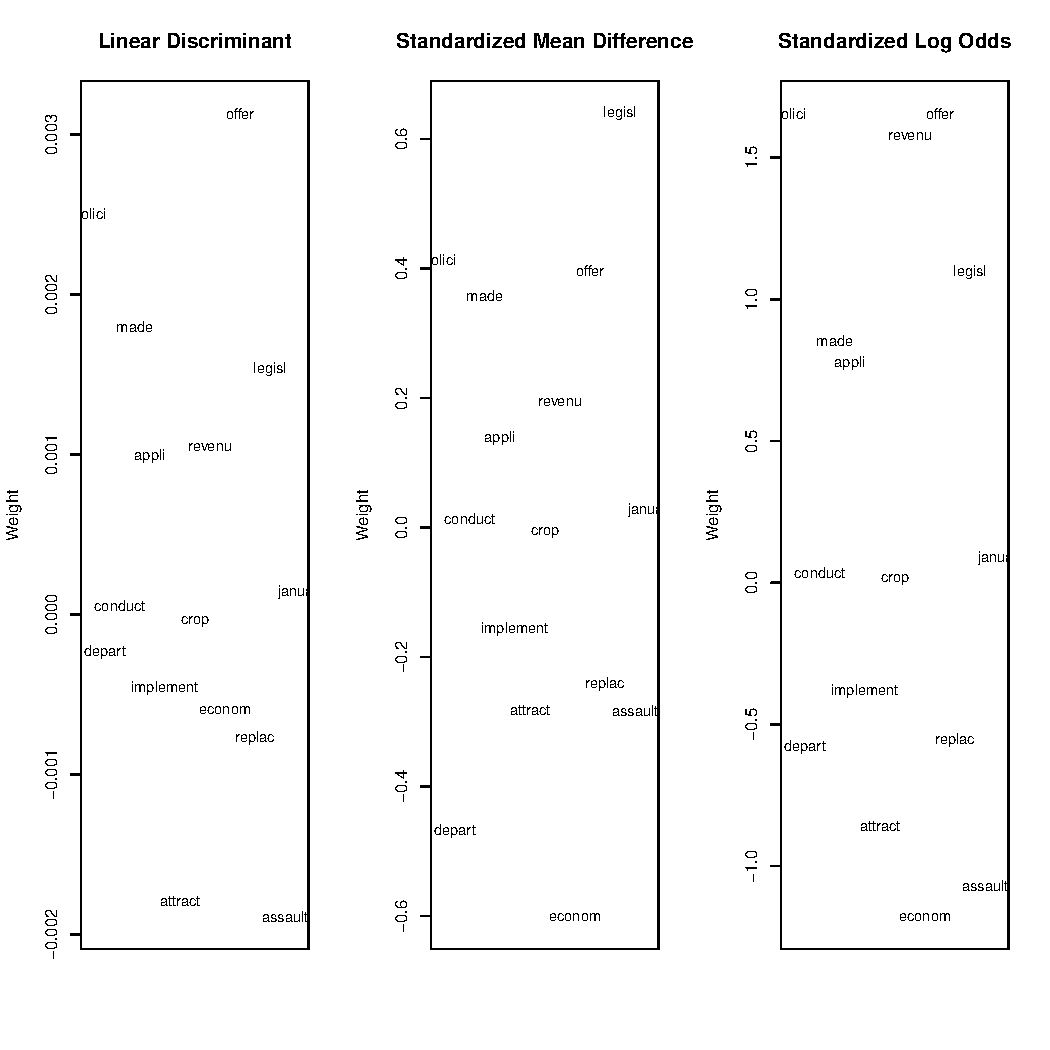
\includegraphics[width=.6\linewidth]{HW2wordDistanceUnigrams.pdf}\\
\end{figure}

\begin{figure}[H]
  \caption{\footnotesize{Word separation measures for trigrams.}}
  \centering
   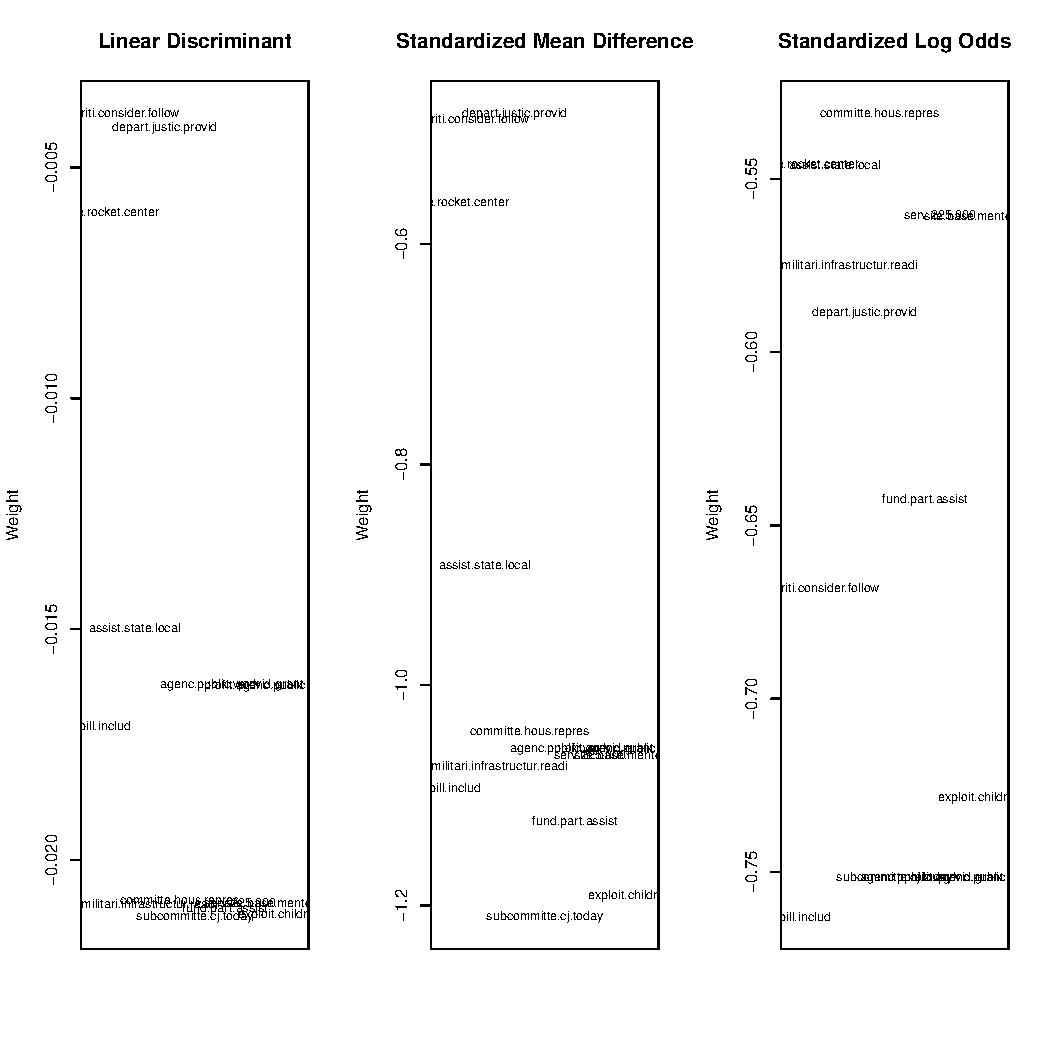
\includegraphics[width=.6\linewidth]{HW2wordDistanceTrigrams.pdf}\\
\end{figure}

\noindent Both senators seem to talk about legislation and politics.

\subsubsection*{Comparing Document Similarity}

Using the trigram word document matrix, let's compare 100 Shelby press releases to 100 Sessions press releases.
\begin{itemize}
\item[1)] Devise a method to sample 100 press releases from each senator's collection
\item[2)] Create the following six matrices:
\begin{itemize}
\item[i)] Euclidean distance between documents
\item[ii)] Euclidean distance between documents with tf-idf weights
\item[iii)] Cosine similarity between documents
\item[iv)] Cosine similarity between documents with tf-idf weights
\item[v)] Normalize the rows of the trigram document term matrix.  For row $i$, 
\begin{eqnarray}
\boldsymbol{x}_{i}^{*} & = & \frac{\boldsymbol{x}_{i}}{\sum_{j=1}^{500} x_{ij}} \nonumber 
\end{eqnarray}
Then apply the {\tt Gaussian} kernel to the normalized matrices
\item[vi)] Use the same normalization, but now with tf-idf weights.  Apply the Gaussian kernel.   
\end{itemize}
\item[3)] Using the matrices, identify the most similar (smallest distance) and dissimilar (greatest distance) press releases.  Read the pairs of press releases---do they appear to actually be similar?  Which method appears to perform best?
\end{itemize}

\lstinputlisting[language=R, firstline=105,]{WUSTL_HW2_JZ.r}

\begin{Verbatim}
# there are a lot of ties, but some reasonable reasonable similar documents were:
> findSimilarDocs(ngkTFIDF)
    row col
941  67  67
> findSimilarDocs(euclideanDistMatrix)
    row col
747  43  36
799  36  43
> findSimilarDocs(ngkTFIDF)
    row col
941  67  67
> findSimilarDocs(cosineTFIDF)
    row col
648  32  32
\end{Verbatim}

\end{document}